%!TEX root = ../../thesis.tex
\chapter{Synchronization}
\label{impl-sync-algorithm}
This chapter explains all details about both the frontend and backend implementation of  Differential Synchronization and the adoptions that were made during the development. 

As discussed in \refchapter{sec:realtime-discussion}, the implementation of the synchronization algorithm is based on WebSockets. The NodeJS module socket.io\footnote{\url{http://socket.io/}, Guillermo Rauch, last checked on 12/03/2014} is used as an abstraction layer on top of raw WebSockets because it adds support for rooms and sending messages in a request-response way, instead of plain one-way WebSocket messages. In addition to socket.io, jsondiffpatch\footnote{\url{https://github.com/benjamine/JsonDiffPatch}, Benjam\'{i}n Eidelman, last checked on 13/02/1014} is used as a key part of the implementation. It is used to create and apply diffs to the underlying JSON data structure on both sites.

\subsection{Protocol}
\label{subsec:ds-algo-protocol}

The synchronization is backed by an own protocol on top of WebSockets (see \refchapter{realtime-ws}), which is modeled after the control flow of the Differential Synchronization algorithm (explained in \reffigure{fig:DiffSync}). Further, the developed protocol adds a new message to the original control flow to make the synchronization more instant.

\begin{figure}[htb]
  \centerline{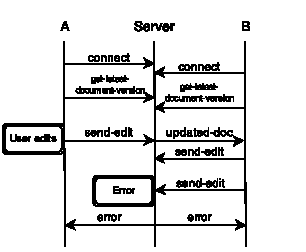
\includegraphics[width=0.8\linewidth]{images/ds-protocol.pdf}}
  \caption[The synchronization protocol]{The synchronization protocol}
  \label{fig:ds-protocol}
\end{figure}

The initial `connect' message leads to the initialization in both server and client. The client sets up a new data structure for the synchronization and the server adds the client to a list of connected clients for the current document.

After the initial `connect' message has been successfully transferred to the server, the client sends a `get-latest-document-version' message to which the server will reply with the newest version of the requested document.

Each edit to a document is transferred in a `send-edit' message which contains a JSON payload of all outstanding edits. The message is created on the client by creating a diff of the server shadow and the client's version of the document. The server will receive that message and apply the diff to the current version of the document and the client's shadow version. A diff payload looks like this:

\begin{lstlisting}[language=JavaScript, caption=Edit Payload, label=lst:edit-payload]
{
  id: "document_id",
  edits: [
    { localVersion: x, serverVersion: y, diff: Object, sum: SHA1 }
  ],
  localVersion: currentLocalV,
  serverVersion: serverShadowV
}
\end{lstlisting}

It contains information about the most recent document versions, the document's id and an array of all edits. Each edit is composed of both the client version and the server shadow version that it is based on. The diff is also part of each edit object, as well as a checksum of the document which is used for sanity checking.

If any error occurs either on the server or the client, e.g. a diff fails, both server and client can send an `error' message which either initiates a reload of all connected clients, if the server sent the `error' message, or a reload of all clients and a refetch of the currently edited document on the server to have a fresh, consistent start after an error. In this way, all connected clients and the server stay in sync, even if an error occurs.

The last message in the protocol, which is not part of the original communication flow, is the `updated-doc' message. It does not have a payload and is used to notify peers about new changes on the server. The function of this message is explained in more detail in \refchapter{subsec:ds-algo-enhancement}.

\subsection{Backend}

The backend keeps an in-memory list of all currently edited documents with all associated client socket connections. Every time a client connects and requests the newest version of a document, the backend creates a new entry in its document list, fetches the requested document from the database and adds a connection to the client to the list. Clients that try to connect to the same document will be added to the client list after the backend has checked if the client is allowed to edit the document. Rejected users are not added to this list and they will see an error message in their frontend. The list of clients is updated every time a client connects or disconnects and in case the last client disconnects, the document is saved one last time and then deleted from the list of managed documents.

The reason why the list of managed documents is not stored persistently is because all operations on that list and on the associated documents need to be done instantly or otherwise there would be more delay between document updates on clients. Also, it is not severe if the data is lost when the server reconnects because the clients will receive `error' messages when they try to update the document after the reload and they will reload afterwards to achieve a consistent state. Further, the data loss is minimal because the server saves the document to the database periodically in short intervals.

\begin{lstlisting}[language=JavaScript, caption=DS implementation (Backend), label=lst:ds-backend]
  function(edit){
    if(versionsMatch(shadowDoc, edit)){
      backupDoc = copy(shadowDoc);
      shadowDoc = applyPatch(copy(shadowDoc), edit);
      serverDoc = applyPatch(copy(serverDoc), edit);

      if(checkSum(shadowDoc, edit.sum)){
        notifyAllPeers();
        saveDocument();
      }else{
        revert();
        sendError();
      }
    }else{
      useBackUpDocument(edit);
    }
  }
\end{lstlisting}

The above code (\reflisting{lst:ds-backend}) demonstrates a simplified version of a part of the Differential Synchronization implementation which is used on the client and on the server. It only shows the part that applies edits to a document and leaves out parts of the version logic (see \refchapter{sync-diffsync}) to shorten the example. Also, the above example is only the server part of the algorithm and contains server-specific naming conventions and some extra steps which are not necessary on the client. The client implementation however is almost identical to the version that is explained here.

It is assumed that the list of edits is sent in order, meaning that the ones who were applied to earlier versions are the first edits in the array. Before applying an edit, the server needs to check if the versions of the edit and the server shadow match (line 2) so that the edit can be applied to the current document. When they do not match, the backup document is used to apply the edit (line 15). If the version matches, the server is able to patch the shadow document and the current server document (line 4f). Before that, the shadow document becomes the new backup document (line 3). This step is left out on the client, because the client does not need to keep backups.

It is important to apply the edit to deep copies of the objects, instead of references to the object, because the patches are applied in-place, meaning that the base objects are changed and therefore all references to the objects point to the same changed object. If for example the new backup document would not be a copied version of the shadow (line 3) and the patch would not be applied to a copy of the shadow document, the backup and the shadow would be the same document because they are referencing the same object reference: \code{shadowDoc}. So instead of backup being the old version of the document's shadow, it would be the exact same object and all future usages of the backup would lead to inconsistent results.

After applying the patch to the different documents, the checksums need to be checked in order to ensure that they were transmitted and applied correctly (line 7). If this fails, all operations need to be reverted and the client needs to reload and start fresh (line 11f). But if all goes right, all other peers are notified about the update and the new version will be saved to the database (line 8f).

When an edit has been applied to a document successfully, \code{saveDocument} is called which will schedule a database write operation within the next second. If there are more write requests in the next second, the operation will be postponed for another second which can be postponed again. This method dramatically reduces the database's write-load which, in case of saving every single document change, can be very high if there are several arrangements edited at the same time. Also, the system ensures that for each arrangement, only one write request is handled at once to reduce the load even more.

Still, the database will have to save many changes to a document over time. Especially when documents are edited simultaneously over a longer time. The load can be handled easily by CouchDB because it is built on top of an append-only B-tree so that document writes are fast and non-blocking \cite[chapter: The Power of B-trees]{anderson2010couchdb}. For each database write, a new version of the document is appended which, in the case of many writes per minute and large document structures, can lead to a quickly growing size of the database. One way to reduce the size of a database is to `compact' it, which means that previous versions of all documents in the database will be removed to make more space. The system is configured to compact the arrangement database once each day if the write load to this database is not too high. A compaction of a database with a high write-load leads to a much slower write performance and is therefore not advised.

\subsection{Frontend}

As mentioned before, the client's patch implementation does not differ much from the server's implementation. The part of the client's implementation in which a diff is created will be explained in this section.

\begin{lstlisting}[language=JavaScript, caption=DS implementation (Frontend), label=lst:ds-frontend]
  if(!isSyncing()){
    var diff = createDiff(copy(shadow), copy(localDoc));

    var editMessage = createMessage();
    editMessage.addEdit(diff);

    applyPatchTo(shadow, diff);

    sendEdits(editMessage);
  }else{
    scheduleSync();
  }
\end{lstlisting}

At first it is important to check if the module is currently syncing (line 1, \reflisting{lst:ds-frontend}), because the algorithm does not allow more than one sync message to be delivered at at time. If the system is syncing at the moment, a new sync iteration is scheduled for after the current sync (line 11). Then, the diff is created from the most recent document (\code{localDoc}) and the \code{shadow} document (line 2). Again it is important to create the diff from object copies, because the diff is later applied to the shadow document (line 7). If the diff would contain references to objects of one of the other documents (e.g. a new object has been added to an array) then all later diff operations would return wrong patches, because the references point to the same objects and changes in these objects would affect both references. Before applying the patch to the local shadow, a new message object is created (see \refchapter{subsec:ds-algo-protocol} for details) and the edit is appended (line 4f). If a previous message exists, e.g. because it could not be delivered, this message is used and the edit is simply added to the edits stack of this message. Lastly, the message is delivered to the server (line 9), which will then trigger the server to send its newest changes to the client again (see \reffigure{fig:DiffSync}).

In addition to the implementation of the synchronization algorithm itself, the frontend also needs a way to detect local changes and to show remote changes in the user interface. Detecting changes locally could be done in two ways. Either the sync-mechanism is manually triggered each time when a value is changed by the user, which would each time require additional and duplicated code. Another way to detect changes is to leverage AngularJS's \code{\$watch} method. All changes to data that are tracked by AngularJS will trigger listeners that watch for changes in the \code{\$rootScope}. In this way, code duplication is prevented and no manual initialization is needed. However, this method also triggers listeners when user interface state changes which does not need to be persisted and therefore creates empty diff messages. Again, the benefit of having an automatic sync-mechanism is more important than preventing sending extra messages to the server.

Propagating remote changes to the application's views turned out to work out of the box because of the way AngularJS handles object changes. After the synchronization of the model is done, a `sync` event is emitted by the \code{\$rootScope} and the arrangement model simply resets its state with the new version. AngularJS's internal object observer will then find out which values changed to update all bindings accordingly and to notify model watchers of the changes.

\subsection{Algorithm Enhancement}
\label{subsec:ds-algo-enhancement}

In the original proposal for Differential Synchronization, the synchronization is only initialized either after the client edited the document or after a specified, probably adaptive, timeout \cite{fraser2009differential}. In a worst case scenario, the timeout happens right before another user edited the document and the client will have to wait for another interval to receive the updated version from the server. One way to overcome this problem is to switch to a peer-to-peer scenario in which each peer is able to notify other peers about its changes\footnote{\cite[p. 4f]{fraser2009differential}}. This would involve a major change of the topology, making it harder to implement and maintain, because a peer-discovery mechanism would be needed through which each peer would find other peers and periodically check if they were still part of the network. Also it would mean that each peer would need to maintain a shadow document for each other peer and the overall computation time would increase. 

Instead of building up a peer-to-peer system to achieve near real-time updates, the existing WebSocket architecture is used to achieve the same effect. Every time a peer sends an edit to the server and the server is able to perform a valid patch, meaning there is no need to send an `error' message (see \refchapter{subsec:ds-algo-protocol}), it will push a notification to all other connected peers. This notification (the `updated-doc' message) triggers a synchronization cycle on each of the clients which in the end leads to a much more instant update of the document than it was possible when waiting on a timeout to receive remote updates. It is important though, that still only one synchronization cycle is happening at a time and that updates or edits that are happening during a synchronization cycle are postponed to be handled after the current cycle. Otherwise the system will loose its stability and it will result in unwanted errors.

One interesting positive side-effect of pushing change notifications is, that diff sizes are reduced and the effort of computing and applying patches is drastically reduced. A negative side-effect however is, that the amount of messages in the client-server communication increases a lot because each edit that is applied on the server will trigger \code{n-1} `updated-doc' messages and also \code{n-1} `send-edit' messages, where \code{n} is the number of connected peers. Most `send-edit' messages might also be empty because those clients might not have applied changes to the local document. Yet, the overhead of sending more messages pays off for having a faster synchronization across all clients.

Moreover, the implementation of the original algorithm in this project is a working proof, that it is also applicable to JSON data structures. In his paper, Fraser claims that the algorithm could in theory be applied to any data structure ``as long as a difference algorithm and a fuzzy patch algorithm are available for the content''\footnote{\cite[p. 5]{fraser2009differential}} but his reference implementation only provides a solution for full-text diffs. During the implementation of the algorithm for JSON objects, the data structure that was used for arrangements has changed drastically to make it work well with JsonDiffPatch. A crucial part is to correctly detect the changes that were made to objects in arrays because they might be moved, added or deleted and all operations might semantically depend on each other. One major issue is, that the diff algorithm needs to be able to uniquely identify objects in arrays in order to keep track of changes. In the first implementations, the arrangement data structure was complex and had inner-object dependencies which made it hard to create semantically correct diffs. So the data structure was reworked in a much simpler way and, most importantly, providing a way to uniquely identify each object in array structures, by assigning `local' ids to them. These ids are created on the client and only assigned after checking if they collide on the current client. The probability of having two clients creating conflicting ids is unlikely because the they are created from several randomly created numbers and hashed with a time code, which is taken from the audio context's current time and the client's local time.

\subsection{Tracked values}
\label{sub:sync-tracked-values}

One important aspect of implementing the synchronization was to decide which values should be synchronized across clients and which should not be synchronized. The basic decision was to find out which values are part of the arrangement's core and therefore need to have the same state on each client and which values only represent the client's user interface state. For example, when two users are editing a drum loop at the same time it would be counterproductive if the currently selected drum part would be synchronized, because both users should be able to edit different parts of the same drum loop at the same time. But, when two users update a buffer at the same time, it is important that these changes are synchronized e.g. when both users drag a different section handle.

For some parts of the application it was not easily distinguishable if a value was part of the arrangement or if it was part of the user interface state. The track user interface for example gives various options to change the volume of the current track: the slider element, the mute button and the solo button. Should their state be synchronized? The volume of individual tracks is important for the overall arrangement and it could be important to mute tracks for a recording because they are not yet finished. But if users work on different tracks simultaneously, they need to be able to mute other tracks in order to concentrate on the current track. For this reason, the state of the mute button and the state of the solo button are not synchronized but the state of the volume slider is. This gives users the ability to customize their track environment independently while the volume information of the track is still preserved.

\subsection{Limitations}

The nature of the editor's local scheduler draws some limitations onto the correctness of the editor's playback. These incorrectnesses only affect the playback of arrangements temporarily and do not influence the correctness of the underlying data structure. The problem is caused by the divergence of the client's documents. It takes some time to propagate all changes to all clients and so the clients might have a slightly different document for a short amount of time. This itself is not a problem and a normal state until the next synchronization cycle is finished but it can have implications on the playback in certain situations. If for example user A edits a pattern in a drum loop and user B is currently playing the arrangement and the pattern that has just been edited by user A is already scheduled, user B's changes will not affect user A's playback. They will only affect the next time this pattern is scheduled. However, the visual representation of the drum machine changes in real time. If only individual notes are altered, the effect of the divergence-related errors in the playback can be ignored because the impact is too slight and unimportant. Yet, if the order of patterns or the position of the drum loop is changed while a user is currently playing an old version of the drum loop, it can lead to more serious playback problems e.g. a pattern is still playing while the next pattern is scheduled to play at the same time. These edge cases could be prevented by stopping the drum loop's playback for user A if its position or pattern order changed but the consequence of stopping the user's playback will badly influence the user experience. Thus, these edge case will not be handled in the initial prototype of the editor. Further user tests have to show if this edge case needs more intervention. It should be noted, that this does not affect other audio nodes like buffers, because they can be stopped and re-scheduled easily without the need of allocating a lot of memory.

\cite[p. 7]{fraser2009differential} describes another limitation of the Differential Synchronization model itself. It lacks support of author attribution and (text-)cursor synchronization which is built into other synchronization frameworks and applications (e.g. Google Docs\footnote{\url{https://docs.google.com}, last checked on 18/03/2014}). It can be argued however, if this is a feature that should be built into the core of a synchronization model or if it should be a feature that should be implemented independently from the synchronization model as an extension. The synchronization model should only provide a solution to the problem of merging and persisting collaborative changes to a document. By reducing the model to its core functions, it becomes application-agnostic and can easily be used in any collaborative application. Additional functionality can be built in addition to this system but it should not interfere with the synchronization model because it adds more points of failure. Another reason not to include more functionality into the base model is that most additional data points do not need to be preserved persistently (e.g. text-cursors).

% \subsection{Transparent Adaption}

% \subsection{Awareness}

% \cite{koren2013sharedediting}
% \cite{minor1993semiasynchronous}
